Similar to other advanced economies, public transfers in Canada has become a major component of inter-generational transfers, complementing transfers between family members.
Through public transfers, individuals transfer wealth from their productive ages to finance consumption during the ages of dependency.
In that sense, the NTA method can be viewed as a crossectionel implementation of the life-cycle hypothesis \citep{Ando:1963ea,Deaton:2005vr}.
According to that hypothesis, Net transfer is positive at younger ages where the individual depends significantly on inflows for its consumption, and outflows are at their lowest levels.
In adulthood, outflows surpass inflows and Net transfer becomes negative as the individual engages in income producing activities.
Finally in retirement ages the individuals turn back to the government to finance the remaining years of their life.
Net transfer becomes positive again and increases to reach its maximal in the final year of life. \autoref{fig:txAge2015}-A shows the age profile of public transfer in Canada for the year 2015 at the individual level.

\vspace{0.7em}\par
On one hand, per-capita inflows are quite similar for natives and immigrants and overlap at almost all ages.
They average \DTLfetch{statex}{sKey}{Inflows2015AveYoung019}{sVal}\$ between birth and age 19, decrease to about \DTLfetch{statex}{sKey}{Inflows2015AveAdult2059}{sVal}\$ between age 20 and 59 and increase by \DTLfetch{statex}{sKey}{2015rate60+}{sVal}\$ for each birthday from age 60 to reach a maximum of \DTLfetch{statex}{sKey}{Inflows2015Ave90}{sVal}\$ just before death.
We can however notice some slight differences between immigrants and natives from age 60 to 70 in favor of immigrants (ie they cost less) and from age 80 and 90 in favor of natives.
While the first is probably related later retirement among immigrants, the reasons for the latter are less obvious and worth investigating in future research.

\vspace{0.7em}\par
Similar to inflows, the age profile of outflows overlap for immigrants and native till age 14 as individuals from both groups have almost no income producing activity during that period.
But unlike inflows, outflows after age 15 are much lower for immigrants than natives.
From \DTLfetch{statex}{sKey}{Outflows2015Immigrants15}{sVal}\$ for immigrants and \DTLfetch{statex}{sKey}{Outflows2015Natives15}{sVal}\$ for natives at age 15, outflows increase rapidly and the trends diverge for the two groups.
Between age 35 and 59, contributions stabilized around \DTLfetch{statex}{sKey}{Outflows2015AveAdult3554Immigrants}{sVal}\$ for immigrants and \DTLfetch{statex}{sKey}{Outflows2015AveAdult3554Natives}{sVal}\$ for natives.
However, the gap reduced slightly while outflows decrease steadily between age 55 and 69 .
Thereafter till the end of life, contributions stabilized around \DTLfetch{statex}{sKey}{Outflows2015AveAdult70Immigrants}{sVal}\$ for immigrants and \DTLfetch{statex}{sKey}{Outflows2015AveAdult70Natives}{sVal}\$ for natives.

\vspace{0.7em}\par
While the per-capita profiles are different but pretty close for immigrants and natives in 2015, the aggregate profile illustrated in \autoref{fig:txAge2015}-B shows different patterns for the two populations, largely due to the difference in their population size.
For instance, natives are responsible for the bulk of public transfers at all ages, especially for the sub population aged less than 10 and between 60 and 70 years old where the gap between the two population sizes are the largest.

\begin{figure}[H]%
  \caption{Public transfer in 2015 for immigrants and for natives}
  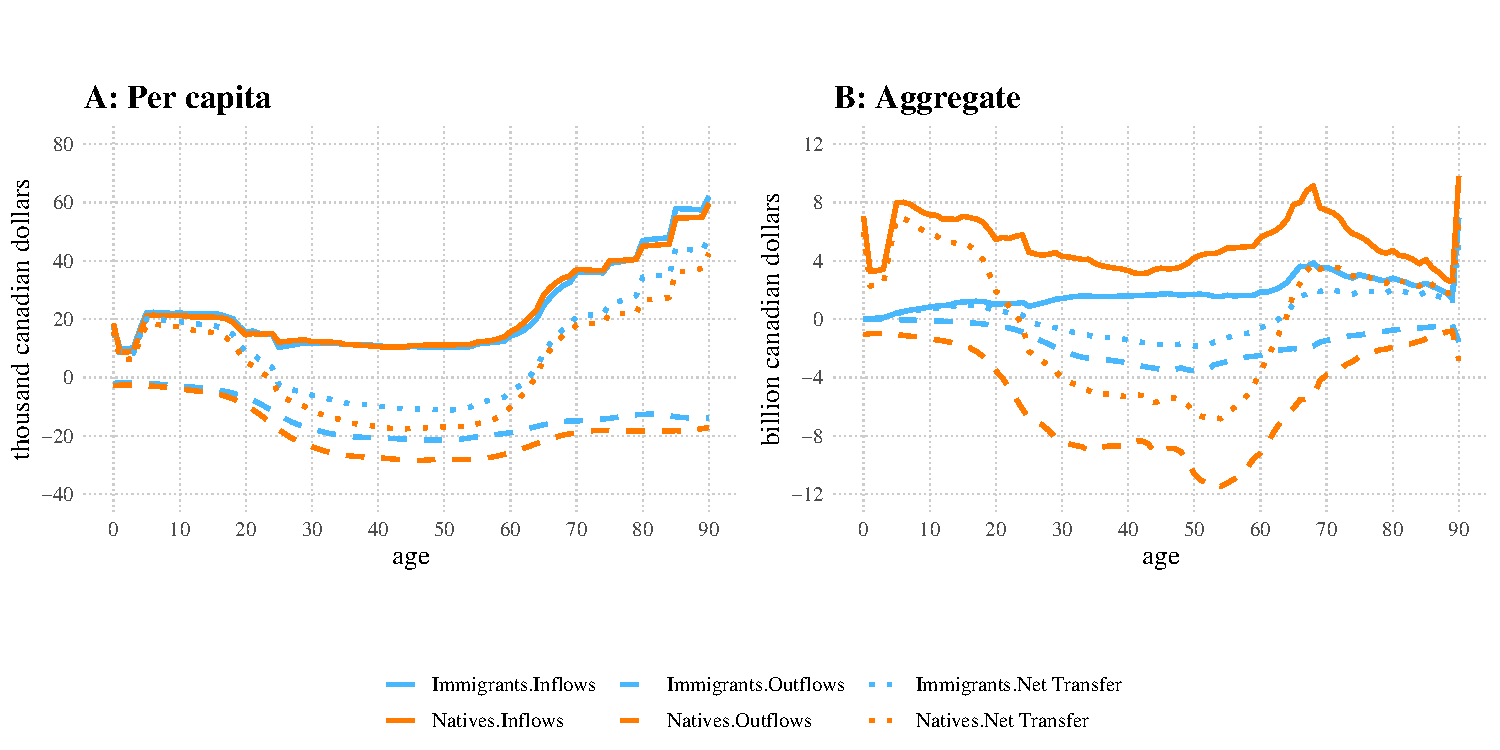
\includegraphics[width=1\textwidth]{res/txAge2015.pdf}%
  \label{fig:txAge2015}%
\end{figure}%